\documentclass{article}
\usepackage[utf8]{inputenc}
\usepackage{graphicx}
\begin{document}
\date{}
\maketitle
\section{Deduplication}

\subsection{How does repeated samples affect the model's predictions?}
\paragraph{Repeated samples can also be seen as the problem of Oversamping.
It is to randomly resample samples of a small number of categories to increase the proportion of this part.Therefore, duplicate data will affect the normal distribution of data.\\So what impact does it have on the prediction of neural networks and the prediction of decision tree classes?\\In model training, the loss function gives the same weight to different samples, so if the sample repetition causes the class imbalance, the model will give a larger weight to the class with more samples.
As an extreme example, of 700 patients with elevated procalcitonin, 500 had severe infection and 300 had no significant symptoms. In order to control the sample balance, 1 out of 300 mild patients was repeatedly sampled, and the data was expanded by 200. The weight learned by such repeated samples is very large, so the mild patient samples are too significant.\\}

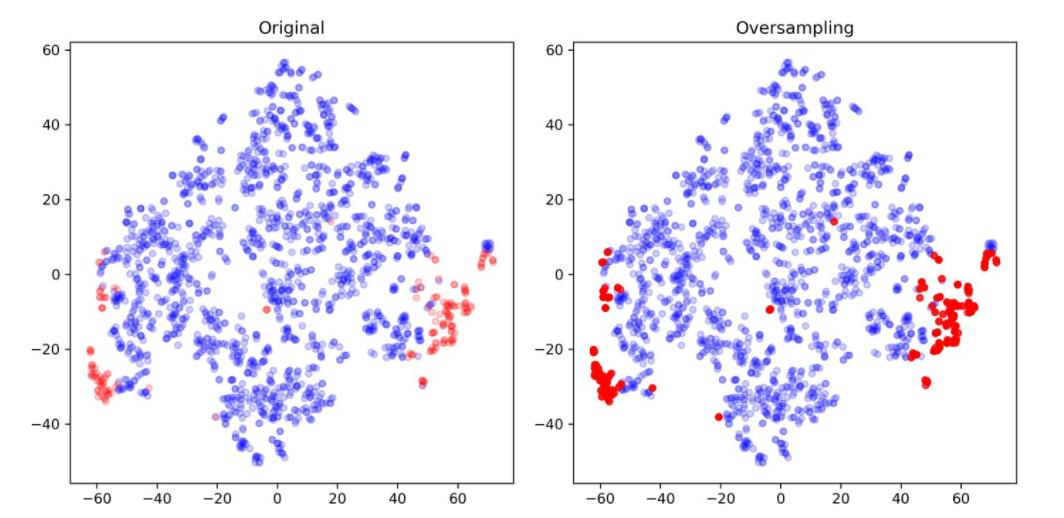
\includegraphics[scale=0.5]{images/oversampling.png}
\paragraph{As shown in the figure: red represents positive examples, blue represents negative examples. Where the data is repeated, the color is darkened.As shown in the figure on the right: there are few positive examples, and when copying a large number of positive examples to join training, it is simply repeating the learning of the positive examples. Therefore, the existing positive examples will be (are) overemphasized.In case some wrong samples or noise are mixed in, the error will be multiplied. So the biggest risk is overfitting.}







% \subsection{Remove duplicate fields, remove duplicate samples (SQL)}
% \paragraph{1.delete from order_info where id not in (select id from (select min(id) as id from order_info group by order_number) as b)\\2.delete from table where id not in (select min(id) from table group by name having count(name)>1) and  id in (select id group by name having count(name)>1)}


% \paragraph{1、

% select * from people where peopleId in (select peopleId from people group by peopleId having count(peopleId) > 1)

% 2、 delete from people where   peopleName in (select peopleName    from people group by peopleName      having count(peopleName) > 1) and   peopleId not in (select min(peopleId) from people group by peopleName     having count(peopleName)>1)

% 3、

% select * from vitae a where (a.peopleId,a.seq) in (select peopleId,seq from vitae group by peopleId,seq having count(*) > 1)

% 4、

% delete from vitae a where (a.peopleId,a.seq) in (select peopleId,seq from vitae group by peopleId,seq having count(*) > 1) and rowid not in (select min(rowid) from vitae group by peopleId,seq having count(*)>1)

% 5、

% select * from vitae a where (a.peopleId,a.seq) in (select peopleId,seq from vitae group by peopleId,seq having count(*) > 1) and rowid not in (select min(rowid) from vitae group by peopleId,seq having count(*)>1) 

% 6.

% update tableName set [Title]=Right([Title],(len([Title])-1)) where Title like '村%'

% 7.

% update tableName set [Title]=left([Title],(len([Title])-1)) where Title like '%村'

% 8.

% update vitae set ispass=-1 where peopleId in (select peopleId from vitae group by peopleId,seq having count(*) > 1) and seq in (select seq from vitae group by peopleId,seq having count(*) > 1) and rowid not in (select min(rowid) from vitae group by peopleId,seq having count(*)>1) 
% }

\section{Duplication of electronic medical records}

\subsection{Illegal copy}
\paragraph{With the development of medical information technology, structured electronic medical recordsEMRs systems have been widely used and developed.
The application of structured EMRs improves the quality of medical record documents, which is conducive to the release and sharing of medical information of patients within the region, as well as the interconnection and collaboration between medical institutions. When the natural language in the EMRs is input into the model as a sample, the structured electronic medical record is also a repeated sample when there is a copy. Some patients with the same disease have exactly the same main complaint, onset process, causes and treatment methods, and even the same punctuation marks. This method of copying medical records is not easy to find from a single medical record.}
\subsection{The checking on duplication of illegal copies of EMRs }
\paragraph{A similarity checking method based on structured electronic medical records, by defining the document template duplication-checking attributes and document segment duplication-checking attributes of structured electronic medical records, and using the minimum similarity ratio string matching (knuth morris pratt, KMP) algorithm to achieve Similar medical records are checked, and the medical records copied illegally by clinicians are found in the medical record documents of the patients' structured electronic medical records}
\subsection{Minimum Similarity Ratio KMP Algorithm}

\end{document}

